\section{The instrument: gTAO-Net}
\label{sec:instrument}

gTAO-Net (gated Tchebichef Attention Ordinal network) is designed as a measuring instrument: each design choice is a switch, so that two configurations can differ in exactly one factor. For a window $x=\{x_k\}_{k=1}^{S}$ with $S$ streams, the logits are
\begin{equation}
  \ell(x)=h\big(F(T(x))+G(x)\big),
  \label{eq:model}
\end{equation}
where $T$ denotes the stream towers, $F$ the fusion operator, $G$ an optional global link and $h$ the ordinal head (Fig.~\ref{fig:arch}).

\begin{figure*}[!t]
\centering
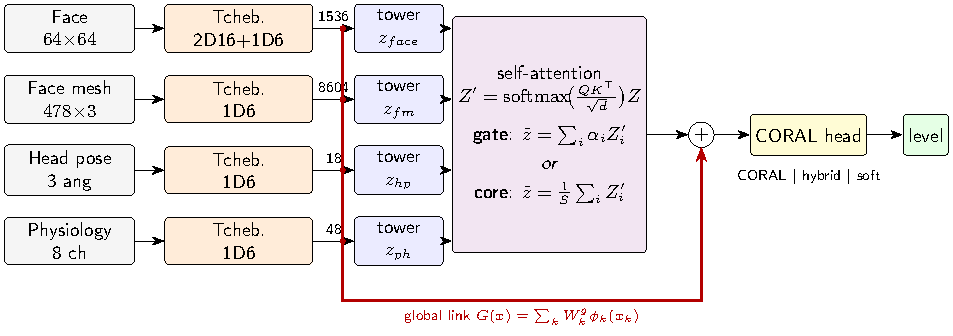
\includegraphics[width=0.72\textwidth]{fig_arch.pdf}
\caption{gTAO-Net. Fixed Tchebichef front-ends $\phi_k$ feed one tower per stream; the tower outputs are fused by a gate or by mean pooling (core); an optional linear global link connects the inputs to the head; a CORAL head is trained with one of three objectives.}
\label{fig:arch}
\end{figure*}

\subsection{Front-ends and towers}
Each stream is a short per-frame sequence. Frames of the image stream are converted to grey $64\times64$ images and projected on the two-dimensional Tchebichef basis of order 16~\cite{mukundan2001tchebichef}. Every image coefficient, landmark coordinate, angle and physiological channel is then projected in time on the one-dimensional basis of order 6. This yields fixed vectors $\phi_k$ of 1{,}536 (frame), 8{,}604 (mesh), 18 (pose) and 48 (physiology) dimensions, which are computed once and cached; no front-end parameter is learned. Our earlier benchmark used Tchebichef coefficients for the face image only~\cite{makhkhas2026ordinal}; here one transform family serves all four modalities, so adding a stream requires choosing a moment order rather than training an encoder. Each tower computes $z_k=\mathrm{LN}(W_2\,\mathrm{GELU}(W_1\phi_k))\in\mathbb{R}^{64}$, with a hidden size of 128 and layer normalisation (LN). A single-stream baseline consists of one tower followed by the head.

\subsection{Fusion}
The stacked tower outputs $Z$ pass through one self-attention step with bias-free query and key projections, $Z'=\mathrm{softmax}(QK^\top/\sqrt{d})Z$. The \emph{gate}, in the spirit of gated multimodal units~\cite{arevalo2017gated}, maps $Z'$ through a two-layer perceptron $g$ to weights $\alpha=\mathrm{softmax}(g(\mathrm{vec}\,Z'))$ and returns $\tilde z=\sum_i\alpha_iZ'_i$; these weights allow it to discard a stream. The \emph{core} variant, following CORE-Net~\cite{tran2026ordinal}, returns the mean $\tilde z=S^{-1}\sum_iZ'_i$ and cannot discard a stream. Following ModDrop~\cite{neverova2016moddrop}, modality dropout removes streams at random during training. Our variant zeroes each tower output with probability 0.2, independently per sample and stream and without rescaling, whereas ModDrop zeroes the inputs of pre-trained modality networks; the global link receives the unmasked inputs.

\subsection{Global link and objectives}
The global link $G(x)=\sum_kW^{g}_k\phi_k(x_k)$ is linear and bias-free. Structurally it is a projection shortcut~\cite{he2016deep} from the inputs to the head. The CORAL head~\cite{cao2020coral} computes $K-1$ logits $\ell_k=w^\top u+b_k$ with shared weights and one bias per threshold, where $u=\tilde z+G(x)$. Three objectives are compared.
\begin{itemize}
\item \textbf{CORAL}: a binary cross-entropy between $\sigma(\ell_k)$ and $\mathbf{1}[y>k]$.
\item \textbf{Hybrid}: inspired by CORE-Net~\cite{tran2026ordinal}, a cross-entropy on the implied class probabilities, plus 0.5 times the CORAL loss, plus 0.1 times a cross-entropy to a neighbour-smoothed target (0.7 on the true class and 0.15 on each neighbour, renormalised at the extremes). Unlike CORE-Net, it has no earth mover's term.
\item \textbf{Soft}: a binary cross-entropy against $t_k=1-\sum_{j\le k}\bar p_j$, the fraction of raters who voted above threshold $k$.
\end{itemize}

\noindent\textbf{Proposition.} If $\bar p$ is one-hot at $y$, then $t_k=\mathbf{1}[y>k]$ and the soft objective equals CORAL.

This is the ordinal counterpart of the observation that single-label learning is a special case of label distribution learning~\cite{geng2016ldl}. It has two consequences. On DAiSEE and EngageNet, where we use one label per sample, soft and CORAL are identical (confirmed bit-identical in the logs). On DIPSER, any difference between them arises from rater disagreement alone.
